\documentclass[compress]{beamer}
\mode<presentation>
{
 \usetheme{Vilanova}
}

\usepackage[english]{babel}

\usepackage[latin1]{inputenc}

\usepackage{times}
\usepackage[T1]{fontenc}

\usepackage{amsfonts}
\usepackage{amsmath}
\usepackage{amssymb}
\usepackage{tikz}
%\usepackage{url}

\title{Pragmatic Remote Sensing}

\subtitle{Image Classification} % (optional)

\author
{J. Inglada\inst{1} , E. Christophe\inst{2}}
\normalsize

\institute[Cesbio, Crisp] % (optional, but mostly needed)
{\inst{1}\textsc{Centre d'�tudes Spatiales de la Biosph�re, Toulouse, France}
\and
\inst{2}\textsc{Centre for Remote Imaging, Sensing and Processing,\\ National University of Singapore}
}

\date{}

\pgfdeclareimage[height=96mm,width=128mm]{background}{fondsClairSansLogo}
\setbeamertemplate{background}{\pgfuseimage{background}}
\pgfdeclareimage[height=0.6cm]{logoIncrust}{logoIncrust}
\pgfdeclareimage[height=0.5cm]{logo_cesbio}{logo_cesbio}
\pgfdeclareimage[height=0.35cm]{logo_crisp}{logo_crisp}
\logo{
\begin{tabular}{lp{0.10\textwidth}lp{0.25\textwidth}r}
\href{http://www.cesbio.ups-tlse.fr/}{\pgfuseimage{logo_cesbio}}\href{http://www.crisp.nus.edu.sg/}{\pgfuseimage{logo_crisp}}
&&\footnotesize{IGARSS 2010, Honolulu}&&
\href{http://www.orfeo-toolbox.org}{\pgfuseimage{logoIncrust}}\\
\end{tabular}
}


\subject{Classification by Example}

% Delete this, if you do not want the table of contents to pop up at
% the beginning of each subsection:
\AtBeginSubsection[]
{
  \begin{frame}<beamer>
    \frametitle{Outline}
    \tableofcontents[currentsection,currentsubsection]
  \end{frame}
}




% If you wish to uncover everything in a step-wise fashion, uncomment
% the following command: 

\beamerdefaultoverlayspecification{<+->}

\begin{document}

\begin{frame}
  \titlepage
{\tiny This content is provided under a Creative Commons
  Attribution 3.0 Unported License} \href{http://creativecommons.org/licenses/by/3.0/}{
\includegraphics[width=0.05\textwidth]{../Ressources/CC-licence.png}}
\end{frame}

\begin{frame}
  \frametitle{Outline of the presentation}
  \tableofcontents[pausesections]
  % You might wish to add the option [pausesections]
\end{frame}


\section[Intro]{What is classification}
\begin{frame}
\frametitle{What is classification}
  \begin{itemize}
  \item Classification is the procedure of assigning a class label to
    objects (pixels in the image)
  \item Supervised
  \item Unsupervised
  \item Pixel-based
  \item Object oriented
  \end{itemize}
\end{frame}

\begin{frame}
  \frametitle{What can be used for classification}
  \begin{itemize}
  \item Raw images
  \item Extracted features
    \begin{itemize}
    \item Radiometric indices: NDVI, brightness, color, spectral
      angle, etc.
    \item Statistics, textures, etc.
    \item Transforms: PCA, MNF, wavelets, etc.
    \end{itemize}
  \item Ancillary data
    \begin{itemize}
    \item DEM, Maps, etc.
    \end{itemize}
  \end{itemize}
\end{frame}

\begin{frame}
  \frametitle{Classification in a nutshell}
  \begin{itemize}
  \item Select the pertinent attributes (features, etc.)
  \item Stack them into a vector for each pixel
  \item Select the appropriate label (in the supervised case)
  \item Feed your classifier
  \end{itemize}
\end{frame}
\section[Unsupervised]{Unsupervised classification}
\label{sec:unsupervised}
\begin{frame}
\frametitle{Unsupervised classification}
  \begin{itemize}
  \item Also called clustering
  \item Needs interpretation (relabeling)
    \begin{itemize}
    \item Class labels are just numbers
    \end{itemize}
  \item No need for ground truth/examples
    \begin{itemize}
    \item But often, the number of classes has to be manually selected
    \item Other parameters too
    \end{itemize}
  \item Examples: k-means, ISO-Data, Self Organizing Map
  \end{itemize}
\end{frame}

\begin{frame}
  \frametitle{Example: K-means clustering}
\setbeamercovered{invisible}

{\tiny
  \begin{center}
    \begin{tabular}{lc}
     \onslide<2->{1. k initial "means" are randomly} &\\
\onslide<2->{selected from the data set.}&\\
&\onslide<2->{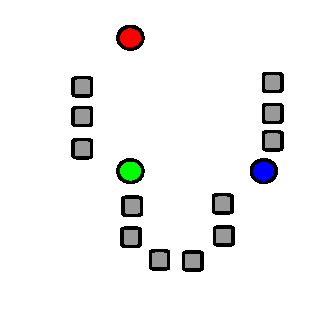
\includegraphics[width=0.15\textwidth]{kmeans_step1.pdf}}\\
     \onslide<3->{2. k clusters are created by associating every} &\\
     \onslide<3->{observation with the nearest mean. The partitions here} & \\
     \onslide<3->{represent the Voronoi diagram generated by the
       means.} & \\
&     \onslide<3->{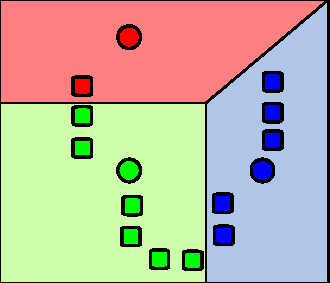
\includegraphics[width=0.15\textwidth]{K_Means_Example_Step_2.pdf}}\\
    \onslide<4->{3. The centroid of each of the k clusters becomes the
      new means.} & \\
&\onslide<4->{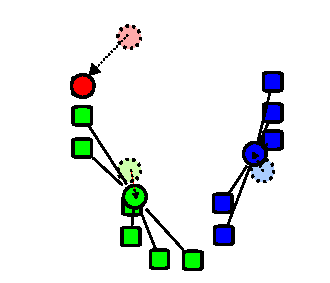
\includegraphics[width=0.15\textwidth]{K_Means_Example_Step_3.pdf}}\\
    \onslide<5->{Steps 2 and 3 are repeated until convergence has been
      reached.} & \\
&\onslide<5->{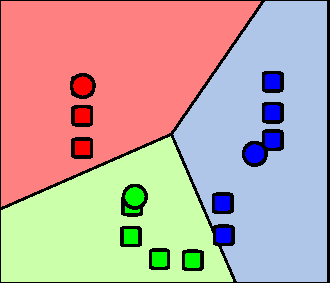
\includegraphics[width=0.15\textwidth]{K_Means_Example_Step_4.pdf}}\\
    \end{tabular}
  \end{center}
{\tiny Image credits: Wikipedia}
}
\end{frame}

\begin{frame}
\frametitle{Example: 5 class K-means }
\begin{columns}
\begin{column}{0.5\textwidth}
\begin{figure}[]
  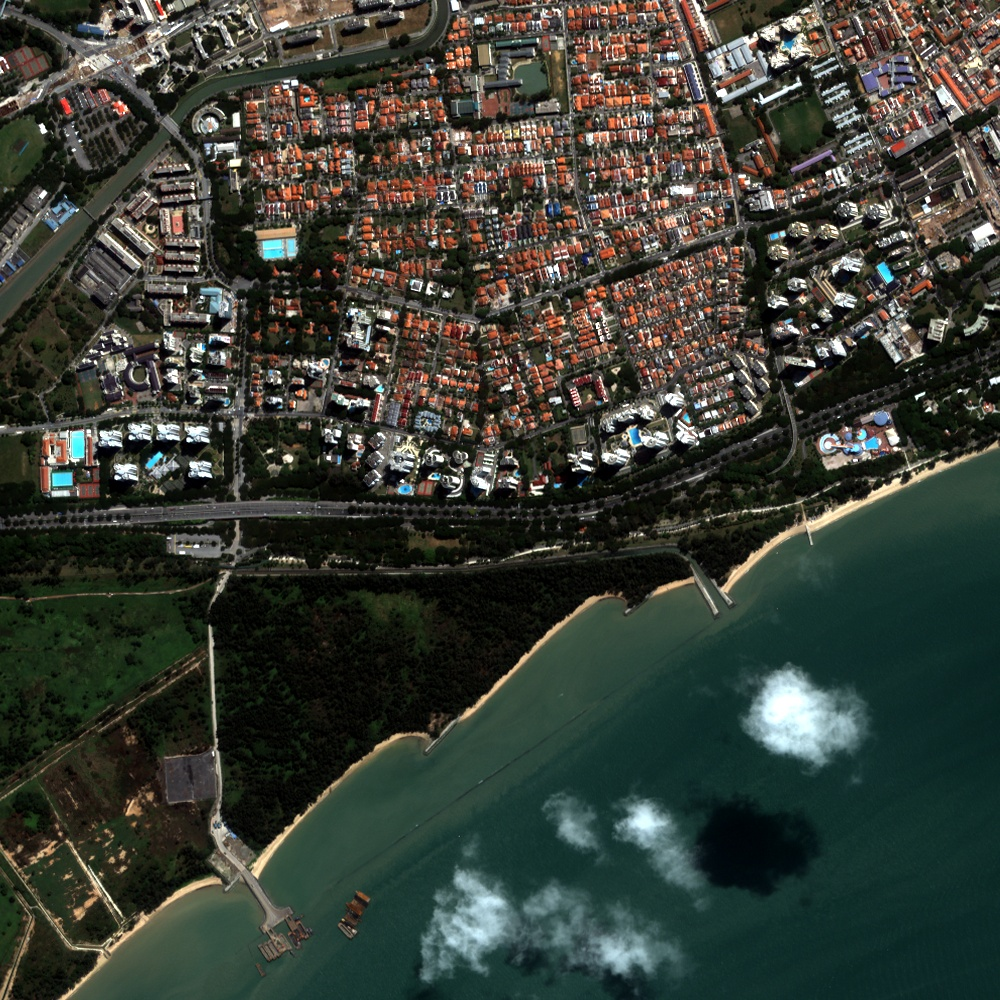
\includegraphics[width=1.0\textwidth]{../03-Features/radio2-extract-3b.jpg}
\end{figure}
\end{column}
\begin{column}{0.5\textwidth}
\begin{figure}[]
  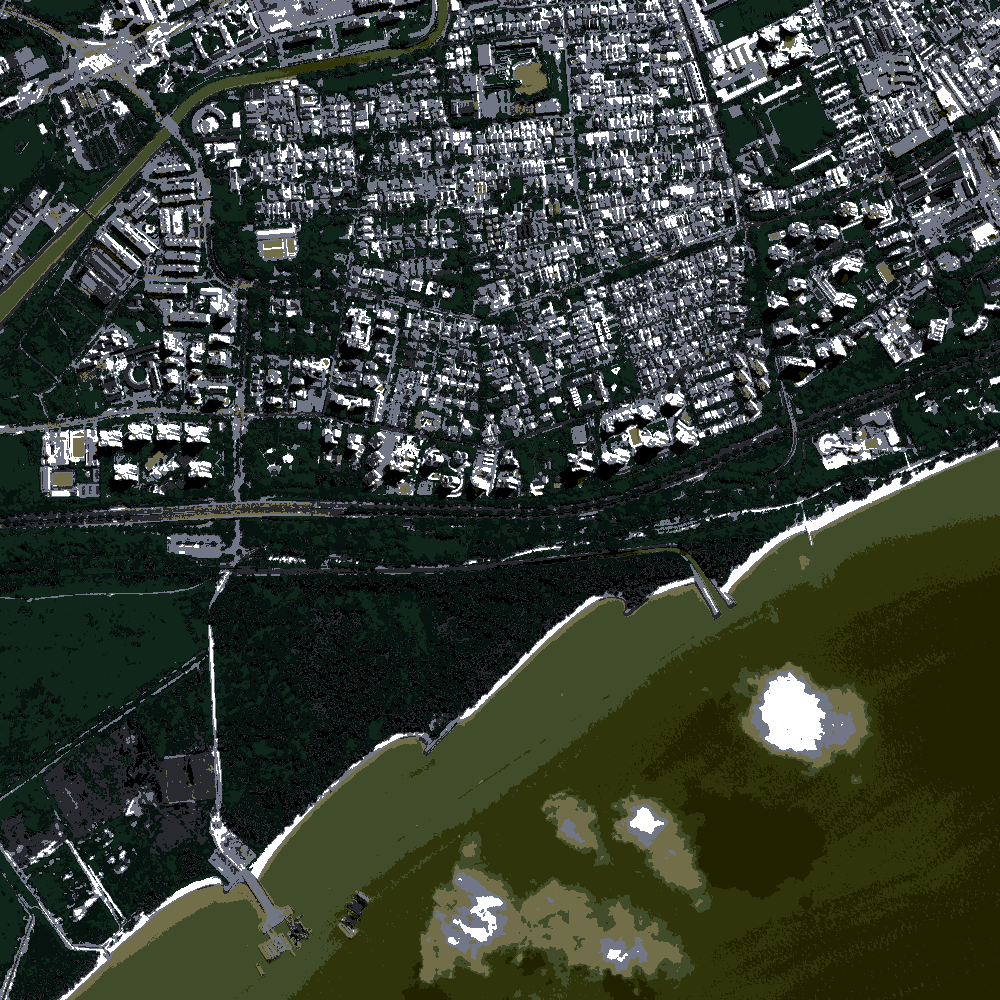
\includegraphics[width=1.0\textwidth]{kmeans-5-classes.png}
\end{figure}
\end{column}
\end{columns}
\end{frame}


\begin{frame}
  \frametitle{Hands On}
  \begin{enumerate}
  \item Monteverdi: Learning $\rightarrow$ KMeans Clustering
  \item Select the image to classify
  \item You can use only a subset of the pixels to perform the
    centroid estimation
  \item Select an appropriate number of classes for your image
  \item Set the number of iterations and the convergence threshold
  \item Run
  \end{enumerate}    
\end{frame}
\section[Supervised]{Supervised classification}
\label{sec:supervised}
\begin{frame}
  \frametitle{Supervised classification}
  \begin{itemize}
  \item Needs examples/ground truth
  \item Examples can have thematic labels
    \begin{itemize}
    \item Land-Use vs Land-Cover
    \end{itemize}
  \item Examples: neural networks, Bayesian maximum likelihood,
    Support Vector Machines
  \end{itemize}
\end{frame}

\begin{frame}
  \frametitle{Example: SVM}
\setbeamercovered{invisible}
{\tiny
\begin{center}
  \begin{tabular}{cc}
\onslide<2->{H3 (green) doesn't separate the 2 classes.} & \onslide<5->{Maximum-margin hyperplane and margins for a} \\
\onslide<3->{H1 (blue) does, with a small margin.} &  \onslide<5->{SVM trained with samples from two classes.}\\
\onslide<4->{H2 (red) with the maximum margin.} & \onslide<5->{Samples
  on the margin are called the support vectors.}\\
& \\
& \\
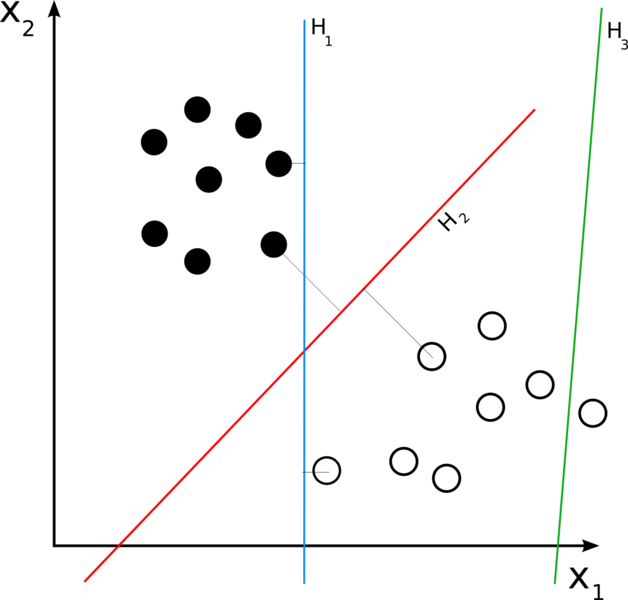
\includegraphics[width=0.3\textwidth]{Svm_separating_hyperplanes.png}
& \onslide<5->{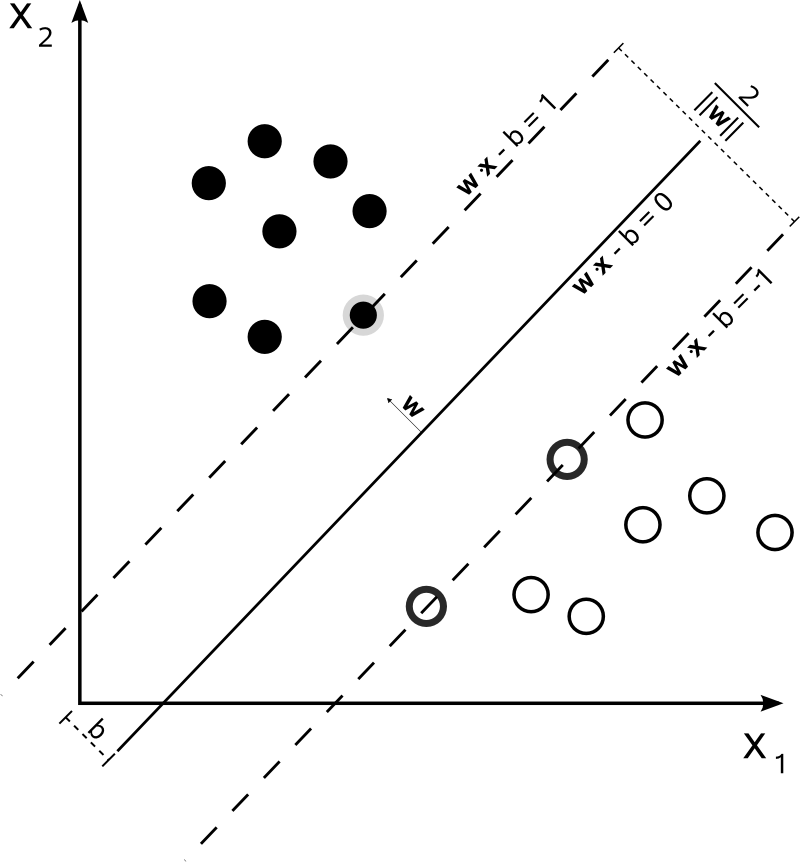
\includegraphics[width=0.3\textwidth]{Svm_max_sep_hyperplane_with_margin.png}}\\
  \end{tabular}
\end{center}
{\tiny Image credits: Wikipedia}
}
\end{frame}

\begin{frame}
\frametitle{Example: 6 class SVM }
\framesubtitle{Water, vegetation, buildings, roads, clouds, shadows}
\begin{columns}
\begin{column}{0.5\textwidth}
\begin{figure}[]
  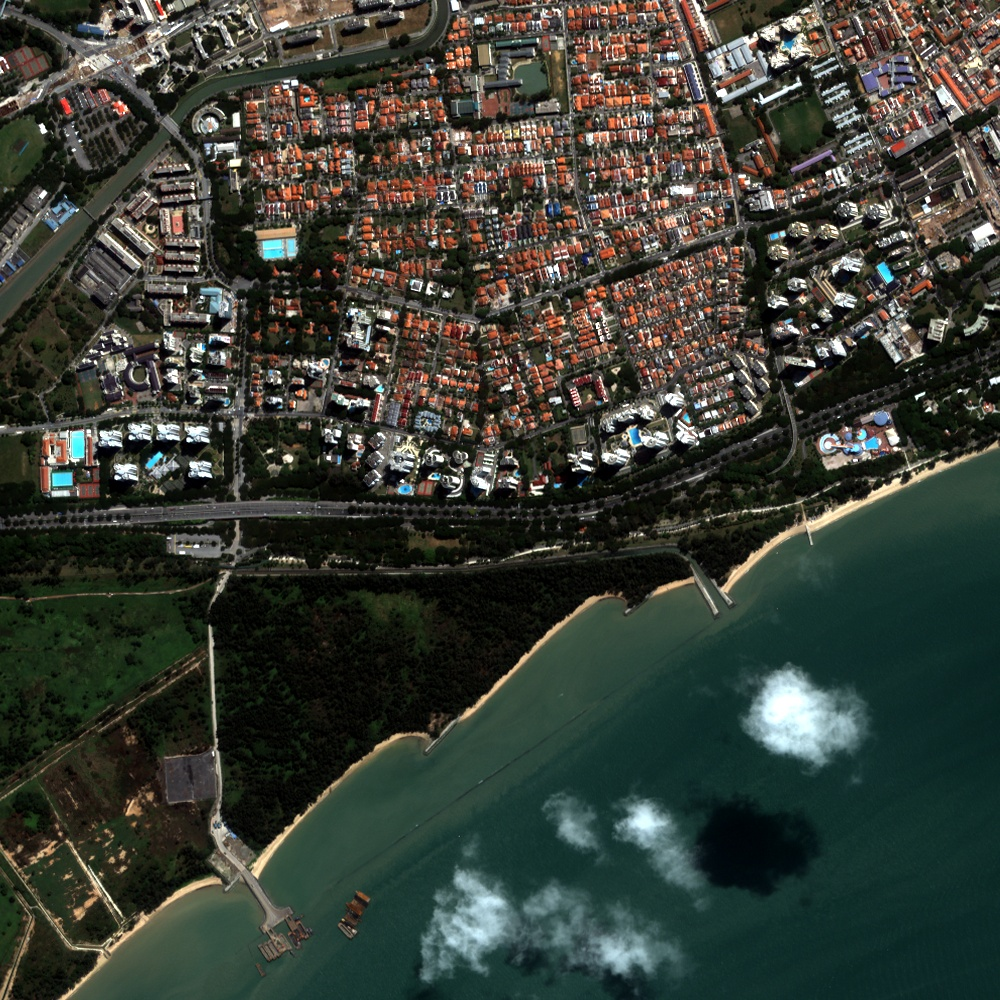
\includegraphics[width=1.0\textwidth]{../03-Features/radio2-extract-3b.jpg}
\end{figure}
\end{column}
\begin{column}{0.5\textwidth}
\begin{figure}[]
  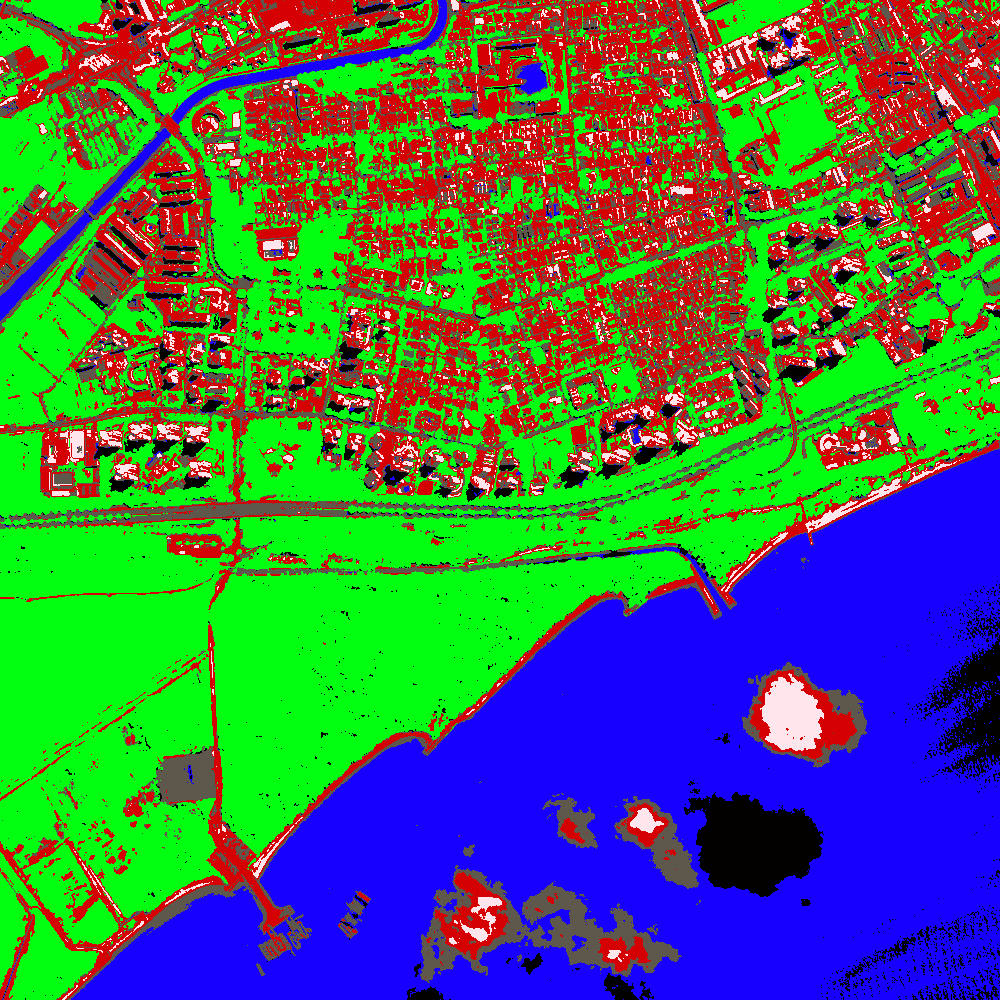
\includegraphics[width=1.0\textwidth]{svm-6-classes.png}
\end{figure}
\end{column}
\end{columns}
\end{frame}


\begin{frame}
  \frametitle{Hands On}
  \begin{enumerate}
  \item Monteverdi: Learning $\rightarrow$ SVM Classification
  \item Select the image to classify
  \item Add a class
    \begin{itemize}
    \item You can give it a name, a color
    \end{itemize}
  \item Select samples for each class
    \begin{itemize}
    \item Draw polygons and use the {\em End Polygon} to close them
    \item You can assign polygons to either the training or the test
      sets; or you can use the random selection
    \end{itemize}
  \item Learn
  \item Validate: displays a confusion matrix and the classification accuracy
  \item Display results
  \end{enumerate}    
\end{frame}

\section[Object oriented]{Object oriented classification}
\label{sec:objectoriented}
\begin{frame}
  \frametitle{Object oriented classification}
  \begin{itemize}
  \item Pixels may not be the best way to describe the classes of interest
    \begin{itemize}
    \item shape, size, and other region-based characteristics may be
      more meaningful
    \end{itemize}
  \item We need to provide the classifier a set of regions
    \begin{itemize}
    \item Image segmentation
    \end{itemize}
  \item And their characteristics
    \begin{itemize}
    \item Compute features per region 
    \end{itemize}
  \item Since individual objects are meaningful, active learning can
    be implemented
    \begin{itemize}
    \item See presentation WE2.L06.2 {\em ``LAZY YET EFFICIENT LAND-COVER
      MAP GENERATION FOR HR OPTICAL IMAGES''}, Wednesday, July 28, 10:25
    - 12:05, by Julien Michel, Julien Malik and Jordi Inglada.
    \end{itemize}
  \end{itemize}
\end{frame}

\begin{frame}
  \frametitle{No hands on}
But a demo if the time allows it!
\end{frame}


\end{document}
